\documentclass[hyperref={pdfpagelabels=false}]{beamer}
\let\Tiny=\tiny
\mode<presentation>{
\usetheme{AnnArbor}
\usecolortheme{beaver}
\usefonttheme{serif}
}
\usepackage{default}
%\usepackage{ucs}
\usepackage[utf8]{inputenc}
\usepackage{gb4e}
\usepackage[T1]{fontenc}
\usepackage{ tipa }
\usepackage{qtree}
\usepackage{synttree}
%\usepackage{color}
\usepackage{tree-dvips}
\usepackage[absolute,overlay]{textpos}
%\usepackage{covington-beamer}
\usepackage{lmodern}
\usepackage{hyperref}
\usepackage{natbib}
\usepackage{graphicx}
\usepackage{eso-pic}
\usepackage{booktabs}
\usepackage{tikz}
%\usepackage{memoir}
%\usepackage{relsize}
%\newcommand{\subscript}[1]{\raisebox{-0.25em}{\smaller #1}}
%\logo{\includegraphics[height=1cm]{nclcbelogomono.eps}}
\setbeamertemplate{footline}[frame number] 
%gets rid of navigation symbols
\setbeamertemplate{navigation symbols}{}

\title{How I learned to stop worrying and love the leave}
\author{Joel C. Wallenberg\\\texttt{joel.wallenberg@ncl.ac.uk}}
\institute{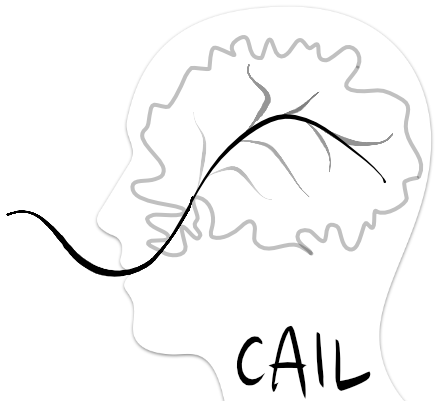
\includegraphics[scale = 0.2]{caillogo.png}}
%\date[]{14th May, 2019}

\begin{document}

\begin{frame}[plain]
\titlepage
\end{frame}

\begin{frame}
	\frametitle{Outline}
	\tableofcontents
\end{frame}


\section{The Meta-Layer}
\begin{frame}{Things people may not tell you about research leave \\(or maybe they're very different to me)} 
\begin{itemize}
	\item So far, I always go in burnt-out. 
		\begin{itemize}
			\item Factor that in, and put down the stick.
			\item[]
		\end{itemize}
	\item I cannot concentrate hard on hard problems all day, nor can I write all day.
		\begin{itemize}
			\item Again, put the stick down.
			\item Working not-full days was still plenty to get out a number of publications, and possibly more effective than working full days.
			\item[]
		\end{itemize}
	\item Good to do some training / personal development / career development that I don't normally feel I have time for.
\end{itemize}
\end{frame}




\section{Some Actual Work}


\begin{frame}{Actual Work: ``Constraints on the Adaptiveness of Information in Language'' (CAIL)} 
	\begin{itemize}
		\item Collaboration with Christine Cuskley and Rachael Bailes
	\end{itemize}
	\begin{center}
		\url{https://cail-project.github.io/}
	\end{center}
\end{frame}

\subsection{Crash Course in Information Theory}

\begin{frame}{Crash course: Information theory and language} 
\begin{itemize}
	\item The amount of information a sender can theoretically communicate about an event is the uncertainty (``entropy'') the receiver has about the event, which may be reduced by a signal.
\end{itemize}
\begin{center}

	\includegraphics[scale=0.55]{../shannonSchematic.png} 


\end{center}

\end{frame}

\begin{frame}{Crash course: Information theory and language} 
	\begin{itemize}
		\item \citet{shannon1948}'s formula for information in an event with \textsl{n} discrete outcomes with probabilities p_1...p_n:
	\end{itemize}
	\begin{center}
		$$\sum_{1}^{n} p_i log_2 \frac{1}{p_i}$$
	\end{center}
	\begin{itemize}
		\item The $log_2 \frac{1}{p_i}$ part is the \textsl{information content} of an outcome.
		\item The unit of information is a \textbf{``bit''}!
	\end{itemize}
	
\end{frame}


\begin{frame}{Crash course} 
\begin{itemize}
	\item The amount of information in a fair coin toss is 1 bit.
	\item The amount of information in an unfair coin toss with $$p = \frac{1}{3}, \frac{2}{3}$$ is less, even though less probable events have higher information content.
\end{itemize}
\begin{center}
	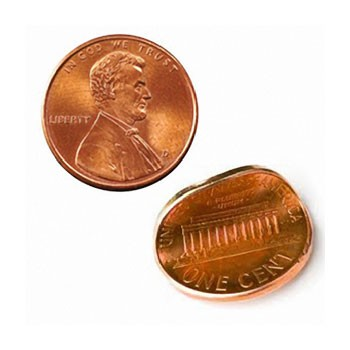
\includegraphics[scale=0.4]{bentcoin.jpg}
\end{center}
\end{frame}





\begin{frame}{``Uniform Information Density'' in language} 
\begin{center}
	``noise'' is any interference, including: noise, memory, other processing costs, etc.\\\vspace*{5mm}
	Speakers spread information content across utterances as uniformly as possible, (possibly) so that utterances are more resistant to noise events \small{\citep{aylettturk2004,levyjaeger2007,levy2008a}}.
\end{center}
\begin{exe}
	\ex How big is the family $[$(that) you cook for$]$?
\end{exe}

\begin{center}
	If \textsl{that} is deleted, more information is carried by \textsl{you}, so information is more dense.
\end{center}


\end{frame}



\begin{frame}{UID and noise resistance} 

\begin{center}
\includegraphics[scale=0.585]{../sentence1info.png} 
\end{center}

\end{frame}

\begin{frame}{UID and noise resistance} 

\begin{center}
	\includegraphics[scale=0.585]{../sentence2info.png} 
\end{center}

\end{frame}


\subsection{Noise resistance and language}

\begin{frame}{Noise resistance experiment} 
\begin{enumerate}
	\item Extract all 10-word sentences from the 1 billion words of EEBO+ECCO combined ($\approx$600,000).
	\item Create alternative versions: random, asymmetric, or optimised (e.g. information hyperdispersed).
	\item A noise event randomly destroys a 3-item sub-sequence.
	\item See how much information the noise events destroy (over 600K trials).
\end{enumerate}
\end{frame}




\begin{frame}{Noise Resistance Experiment: bits lost > 50\%} 


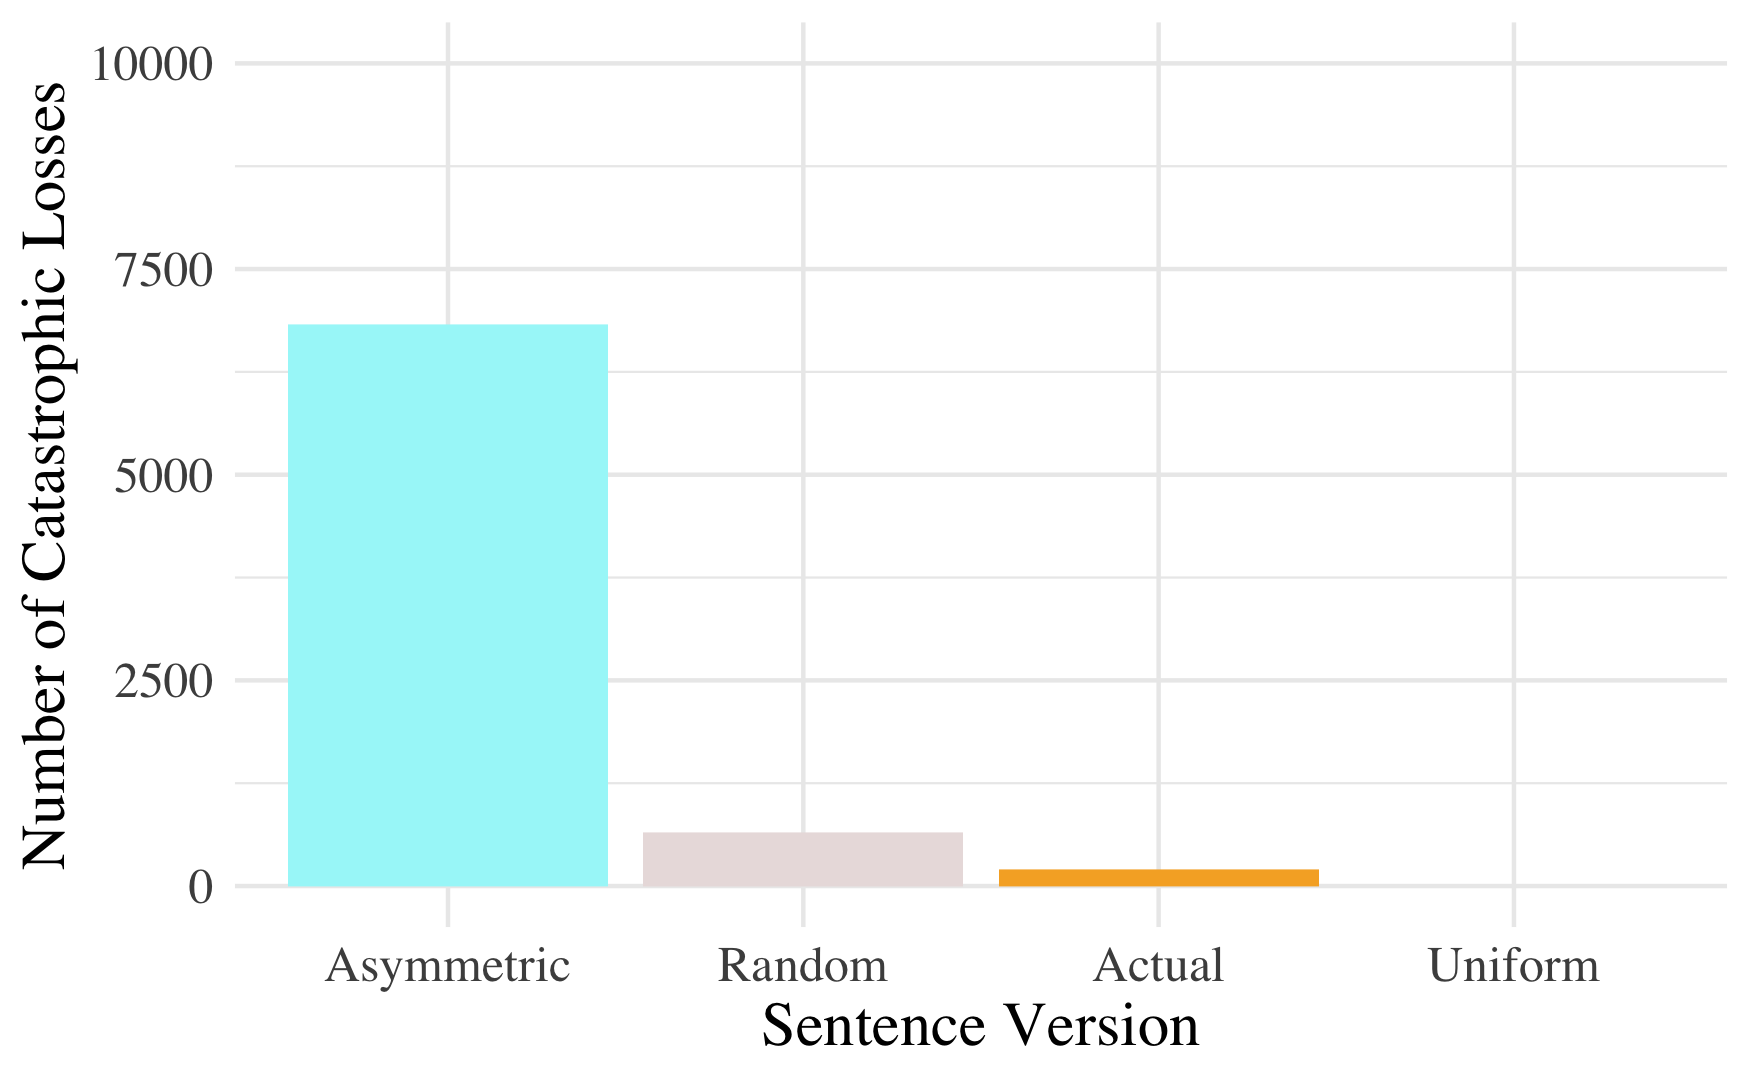
\includegraphics[width=1.07\textwidth]{barplotpyccle.png}

\end{frame}






\begin{frame}[allowframebreaks]
\frametitle{References}
\newcommand*{\newblock}{natbib}
\bibliographystyle{linquiry2}
\bibliography{joelrefs}
\end{frame}




\end{document}